% \draw [conv] (70,126) -- (82,108) -- (107,108) -- (95,126) -- cycle; % Top face
% \draw [conv] (95,126) -- (107,108) -- (107,156) -- (95,174) -- cycle; % Right face

\newsavebox{\conv}

\begin{lrbox}{\conv}
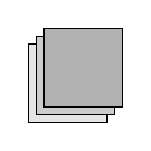
\begin{tikzpicture}
    %   Define 3 squares one behind the other
    \node[draw=black, rectangle, fill=gray!20, minimum width=1cm, minimum height=1cm] {};
    \node[draw=black, rectangle, fill=gray!40, xshift=0.1cm, yshift=0.1cm, minimum width=1cm, minimum height=1cm] {};
    \node[draw=black, rectangle, fill=gray!60, xshift=0.2cm, yshift=0.2cm, minimum width=1cm, minimum height=1cm] {};
\end{tikzpicture}
\end{lrbox}

\newsavebox{\dense}

\begin{lrbox}{\dense}
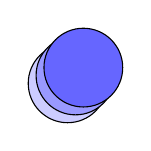
\begin{tikzpicture}
    %   Define 3 circles one behind the other
    \node[draw=black, circle, fill=blue!20, minimum size=1cm] {};
    \node[draw=black, circle, fill=blue!40, xshift=0.1cm, yshift=0.1cm, minimum size=1cm] {};
    \node[draw=black, circle, fill=blue!60, xshift=0.2cm, yshift=0.2cm, minimum size=1cm] {};
\end{tikzpicture}
\end{lrbox}

\newsavebox{\pool}

\begin{lrbox}{\maxpooling2d}
